\chapter{Research}
\label{Chapter:Research}

\section{Related Work}
\subsection{Abuse Detection}
\subsection{Content Filtering}
\subsection{Content Recommendation}
\subsection{Reputation Scoring}

\section{Existing System}
\subsection{Facebook}
\subsection{Twitter}
\subsection{Reddit}

\section{Technologies}
When developing a web application, it is important to explore the range of technologies already available in order to speed up the development process. For this reason, several third party technologies were used to provide some of the core functionality of the system. These technologies include but are not limited to jQuery, Laravel and Google Maps. In addition to the third party technologies, the latest web development technologies were also employed to provide the essential and basic functionality of a web application.

\subsection{Web Technologies} \label{Section:Web_Technologies}

\subsubsection{HTML} 
Hyper Text Markup Language (HTML) is a markup language used for structuring and presenting content on the world wide web \cite{W3:HTML5}. HTML 5 is the recommended standard by W3 as of October 28, 2014 and as such will be used to structure the web application being developed. HTML in itself cannot be used to change the style of page as it was only designed for defining the structure of a page but fortunately HTML tags can be styled. 

\subsubsection{CSS} 
Cascading Style Sheets (CSS) is a simple mechanism for adding style (e.g. fonts, colours, spacing) to Web documents \cite{W3:CSS}. CSS3 is the latest evolution of the Cascading Style Sheets language and aims at extending CSS2.1. It brings a lot of long-awaited novelties, like rounded corners, shadows, gradients, transitions or animations, as well as new layouts like multi-columns, flexible box or grid layouts \cite{Mozilla:CSS3}. CSS3 is being used in this project as it provides a much larger range of styles which are required by Bootstrap.

\subsubsection{JavaScript}
JavaScript (JS) is a high-level, lightweight, interpreted, programming language with first-class functions \cite{Mozilla:JavaScript}. Although JavaScript is not a necessary requirement, it offers many advantages such as allowing manipulation of the document structure after the page has been loaded. As a result of this, one can add, remove or animate content on the page. Inarguably, the main advantage of JavaScript is that it is interpreted on the client side which means less processing is done on the server. This allows for faster loading times as parts of the document can be loaded later, on demand, when required. Collectively, all these and more features improve the user experience and provide a good reason to incorporate JavaScript into a web app.

\subsubsection{PHP} PHP is...\cite{PHP:Home}

\subsection{Frameworks}

\subsubsection{Model-View-Controller (MVC)}
Initially, as stated in the project specification, the system was to be designed as a web based application implemented using the four basic web technologies mentioned previously in section \ref{Section:Web_Technologies}. After completing the initial setup and some implementation, this approach was challenged and a decision was made to find an alternative approach. One of the main reasons for this change in approaches was the overwhelming amount of code that was duplicated across pages making it difficult to make changes whilst maintaining consistency across the pages. As a result, it was decided that a Model-View-Controller approach should be used and implemented using an existing framework.

\begin{figure}[H]
  \centering
  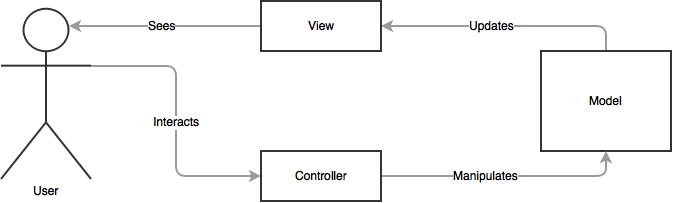
\includegraphics[width=1.0\textwidth]{Images/Technologies/MVC}
  \caption{Information Exchange in an MVC Application.} \label{fig:MVC} 
\end{figure}

The Model-View-Controller (MVC) pattern separates the modelling of the domain, the presentation, and the actions based on user input into three separate classes \cite{MSDN:MVC}. A description of each section as well a graphical representation of communication, figure \ref{fig:MVC}, is given above.

\begin{itemize}
	\item \textbf{Model.} The model manages the behaviour and data of the application domain, responds to requests for information about its state (usually from the view), and responds to instructions to change state (usually from the controller) \cite{MSDN:MVC}. In essence the model is responsible for all interaction with the database and contains any code that either queries or updates records in the database along with some output formatting.
	\item \textbf{View.} The view manages the display of information \cite{MSDN:MVC}. The advantage of this approach is that repeated content can be split into separate views with placeholders and then included by passing in parameters to fill the placeholders. This means that the developer only needs to change the code in one place, particularly useful for things such as navigation and foorter which are consistent across pages.
	\item \textbf{Controller.} The controller interprets the mouse and keyboard inputs from the user, informing the model and/or the view to change as appropriate \cite{MSDN:MVC}. This is where majority of the logic and PHP code for the application is written. Any algorithms and data pre-processing or post-processing methods are written inside the controller.
\end{itemize}

\subsubsection{Laravel}
Laravel, an open-source PHP web application framework intended for the development of web applications following the MVC architectural pattern, developed by Taylor Otwell, was chosen after researching various frameworks \cite{Laravel:Home}. Laravel was chosen over other frameworks for a number of reasons. Not only does it provide an implementation of the MVC pattern, but it also allows allows the user to define custom routes and decide where each route leads rather than having the URL be determined by the file path. Additionally, Laravel comes with solutions to a lot of common tasks and problems straight out of the box making it easier to develop the system straight away without having to ``reinvent the wheel''.

\subsubsection{jQuery} 
jQuery is a fast, small, and feature-rich JavaScript library \cite{jQuery:Home}. It will be used over standard JavaScript as it makes things like HTML document traversal and manipulation, event handling, animation, and Ajax much simpler with an easy-to-use API that works across a multitude of browsers \cite{jQuery:Home}. Although jQuery doesn't necessarily provide any additional functionality over JavaScript as it is powered by JavaScript, it provides shorter notations for common JavaScript functions and provides implementation of features that are lacking in JavaScript, or take long to implement. It can be setup and used by simply including a single script in the document.

\subsubsection{Bootstrap} 
Bootstrap is the most popular HTML, CSS, and JS framework for developing responsive, mobile first projects on the web \cite{Bootstrap:Home}. The main advantage of using Bootstrap is that it easily and efficiently scales your websites and applications with a single code base, from phones to tablets to desktops with CSS media queries. Additionally Bootstrap comes with a whole range of HTML, CSS and jQuery components, that have been pre-styled, further speeding up the development process.

\subsection{Storage}
One of the most fundamental parts of the system is retaining the data that the users enter into the system. There are two different storage solutions for storing and querying the data provided by users. These are both discussed below.

\subsubsection{MySQL} 
MySQL is an open source database management system used for managing data held in a relational database management system (RDBMS) \cite{MySQL:Home}. An SQL database will be used to store all textual information entered by the users. This includes user information, location data, item details and any other necessary information. SQL databases are not encrypted and hence any user credentials such as password will be stored in an encrypted format to prevent access to user accounts in case of a breach.

\subsubsection{Resources}
Along with textual input, it is also necessary to store the images associated as photos with posts, uploaded by the users. One approach to this could be to convert the file to binary and store the binary data in the SQL database. However this approach would lead to the database rapidly growing in size and in turn affecting the performance. Not only would queries take longer to execute but also increase page load times due to the large record sizes. Another approach would be to store any uploaded files either on a storage server or on the web server so they are available on demand. This would result in faster loading time for pages containing these resources as they do not have to be transferred over the network. Due to this, the latter approach will be used during development.